\documentclass[aspectratio=169]{beamer}
\usepackage{color}
\newenvironment{greytext}{\color{gray}}{\ignorespacesafterend}
%
% Choose how your presentation looks.
%
% For more themes, color themes and font themes, see:
% http://deic.uab.es/~iblanes/beamer_gallery/index_by_theme.html
%
\mode<presentation>
{
  \usetheme{default}      % or try Darmstadt, Madrid, Warsaw, ...
  \usecolortheme{default} % or try albatross, beaver, crane, ...
  \usefonttheme{default}  % or try serif, structurebold, ...
  \setbeamertemplate{navigation symbols}{}
  \setbeamertemplate{caption}[numbered]
} 

\usepackage[english]{babel}
\usepackage[utf8x]{inputenc}

\title[]{Stochastic variational inference \\ Structured stochastic variational inference}
\subtitle{CIS 620 paper discussion}
\author{Simeng Sun}
\date{Oct. 9th, 2018}

\begin{document}

\begin{frame}
  \titlepage
\end{frame}

% Uncomment these lines for an automatically generated outline.
%\begin{frame}{Outline}
%  \tableofcontents
%\end{frame}


\section{Outline}

\begin{frame}{Outline}

    \begin{itemize}
      \item A quick review of mean-field variational inference
      \item Traditional coordinate ascent algorithm
      \item Stochastic variational inference(SVI)
      \item Structured SVI
    \end{itemize}
    

\end{frame}

\begin{frame}{Outline}

    \begin{itemize}
      \item A quick review of mean-field variational inference
      \begin{greytext}
      \item Traditional coordinate ascent algorithm
      \item Stochastic variational inference(SVI)
      \item Structured SVI
      \end{greytext}
    \end{itemize}

\end{frame}

\begin{frame}{Variational Inference}
    \begin{figure}
        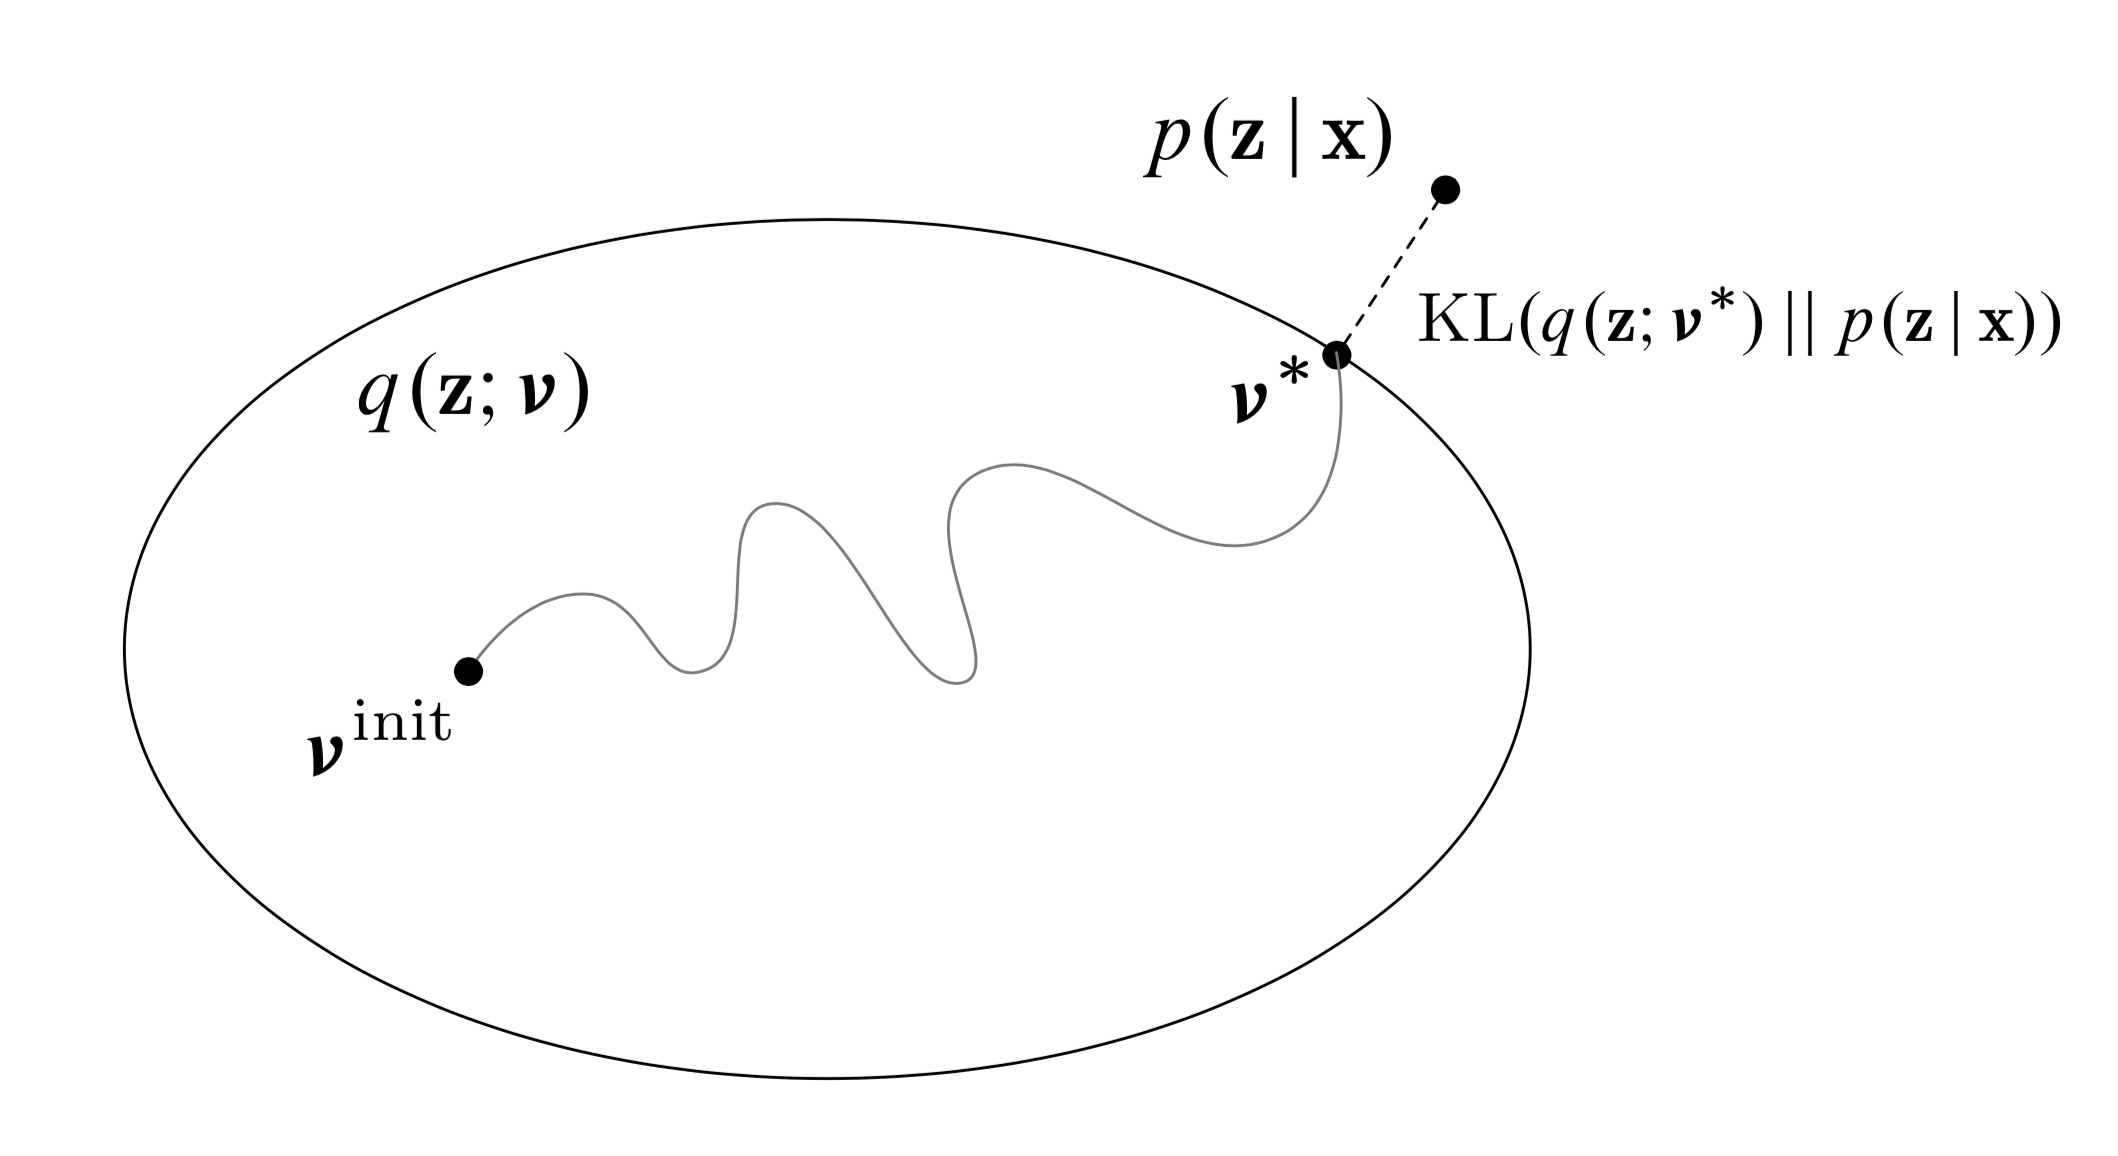
\includegraphics[width=0.65\textwidth]{VI.png}
    \end{figure}
    \begin{center}
        $p(\textbf{z}|\textbf{x})$ true posterior distribution\\
        $q(\textbf{z};\textbf{v})$ tractable variational posterior distribution\\
        Minimize the Kullback–Leibler divergence
    \end{center}
    \footnotetext[1]{pic from https://media.nips.cc/Conferences/2016/Slides/6199-Slides.pdf}
\end{frame}

\begin{frame}{Variational Inference - setup}
    
    \begin{columns}
    \begin{column}{0.48\textwidth}
        \begin{figure}
        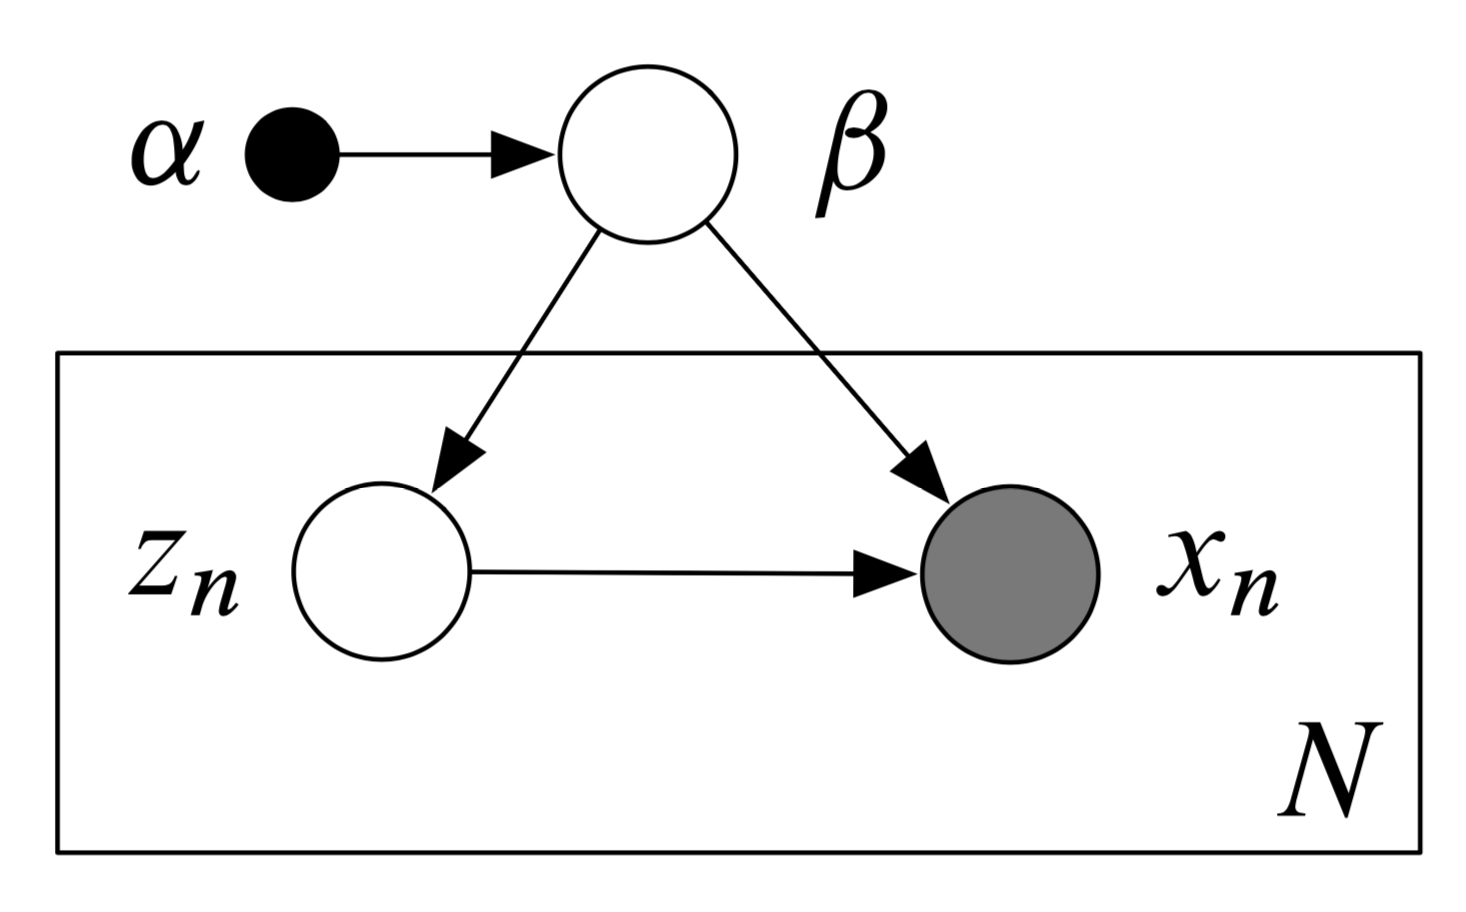
\includegraphics[width=\textwidth]{setup.png}\hspace*{12cm}
        %% add some description of this graph
        \end{figure}
    \end{column}
    \begin{column}{0.48\textwidth}
        \begin{block}{Variables}
        $\alpha$: fixed parameters\\
        $\beta$: global hidden variables\\
        $x_n$: $n^{th}$ observation\\
        $z_n$: context of $n^{th}$ observation ($z_{n,1:J}$)\\
        $z_{n,1:J}$: set of $J$ local hidden variables 
        % exponential family
        \end{block}
    \end{column}
    \end{columns}
    \footnotetext[1]{pic from http://www.columbia.edu/~jwp2128/Papers/HoffmanBleiWangPaisley2013.pdf}
\end{frame}

\begin{frame}{Variational Inference - setup}
    
    \begin{columns}
    \begin{column}{0.48\textwidth}
        \begin{figure}
        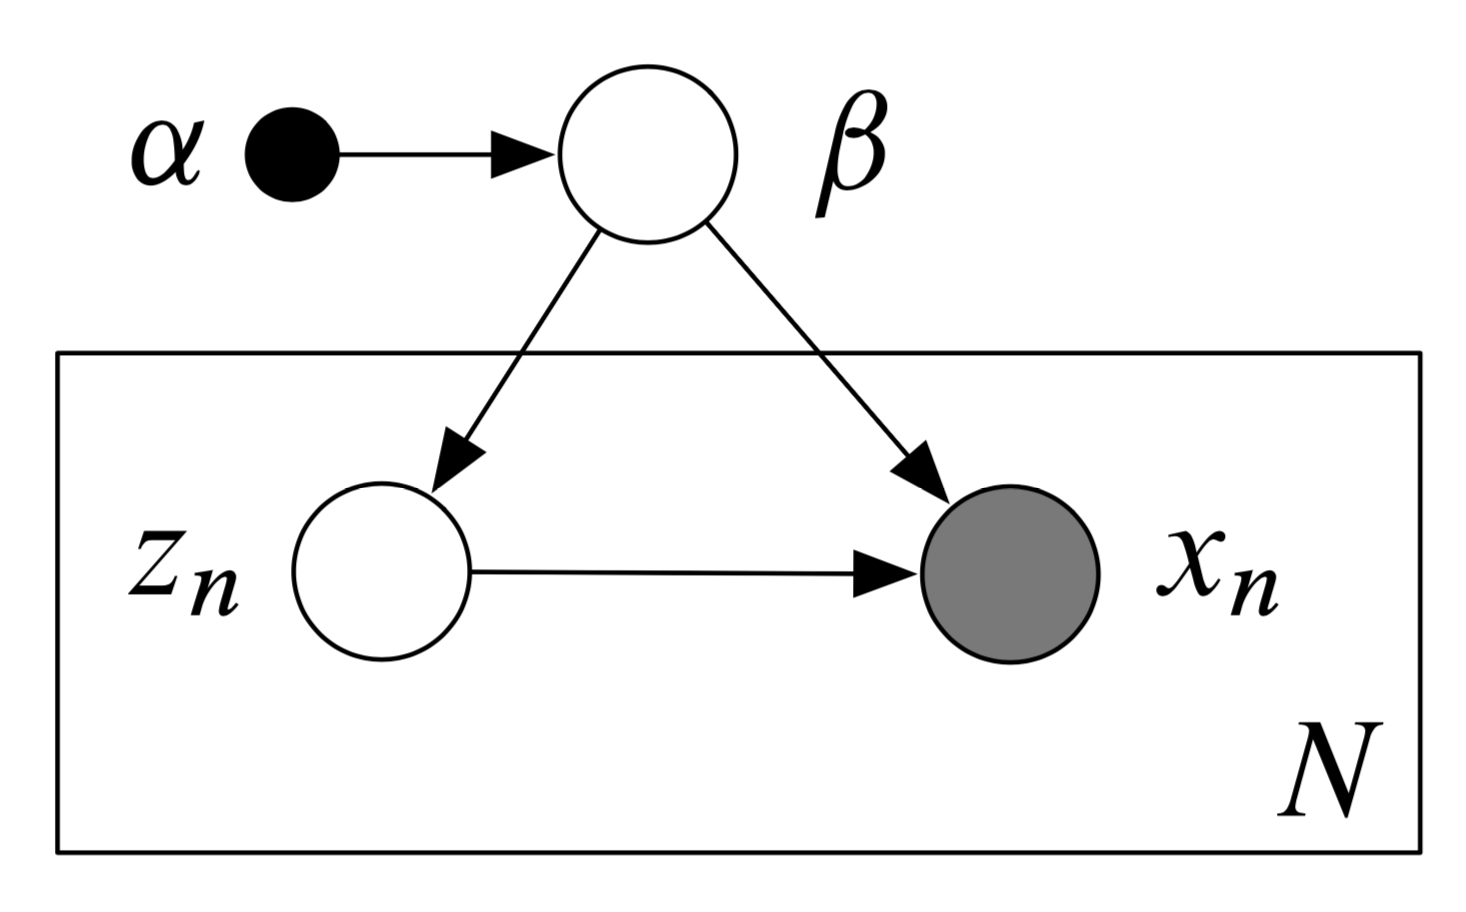
\includegraphics[width=\textwidth]{setup.png}\hspace*{12cm}
        %% add some description of this graph
        \end{figure}
    \end{column}
    \begin{column}{0.48\textwidth}
        \begin{block}{Assumptions}
        \begin{itemize}
            \item Independence of hidden variables (\textbf{Mean-Field})
            
        \end{itemize}
        \end{block}
    \end{column}
    \end{columns}
    \footnotetext[1]{pic from http://www.columbia.edu/~jwp2128/Papers/HoffmanBleiWangPaisley2013.pdf}
\end{frame}

\begin{frame}{Mean-Field Variational Inference}
    
    \begin{columns}
    \begin{column}{0.48\textwidth}
        \centering
        \textbf{Model dependencies}
    \end{column}
    \begin{column}{0.48\textwidth}
        \centering
        \textbf{(Naive) Mean-Field dependencies}\\
    \end{column}
    \end{columns}
    
    \begin{columns}
    \begin{column}{0.48\textwidth}
        \begin{figure}
        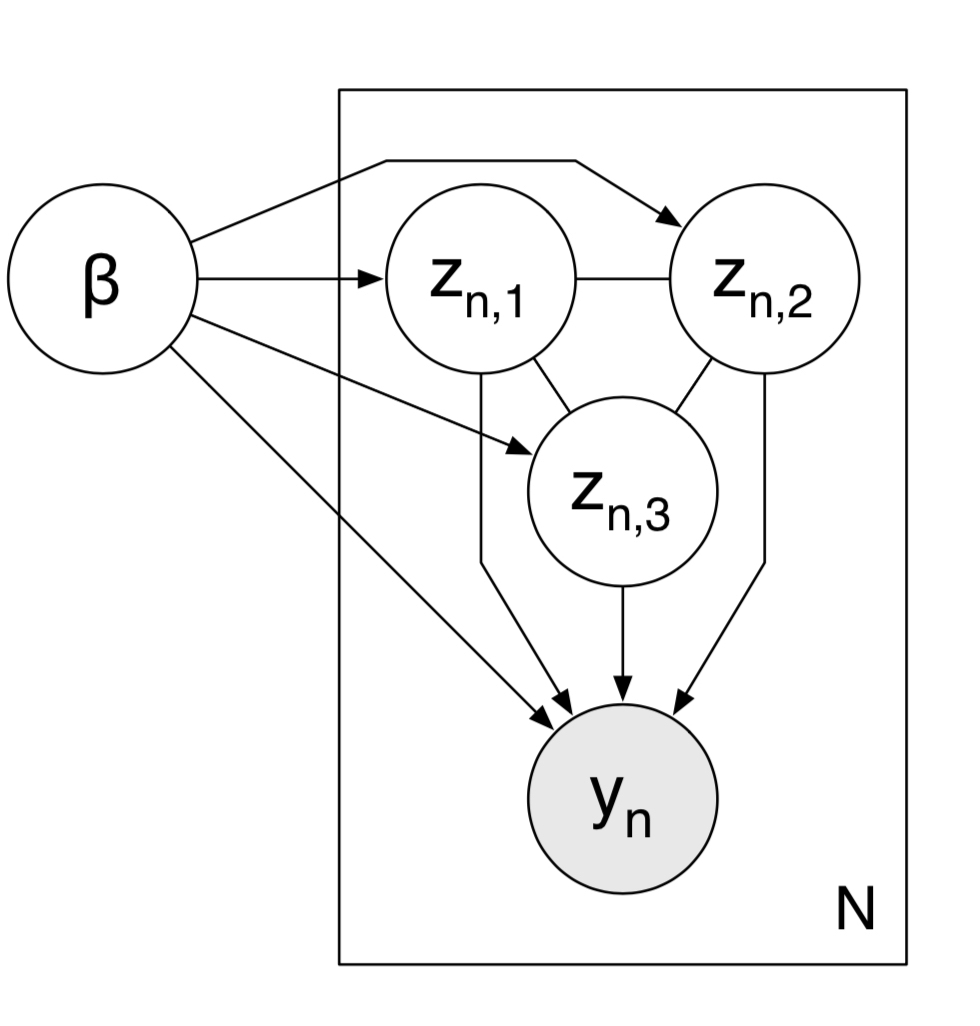
\includegraphics[width=0.8\textwidth]{model_dep.png}\hspace*{12cm}
        \end{figure}
    \end{column}
    \begin{column}{0.48\textwidth}
        \centering
        Intractable posterior distribution becomes a distribution where all variables are independent
        \begin{figure}
        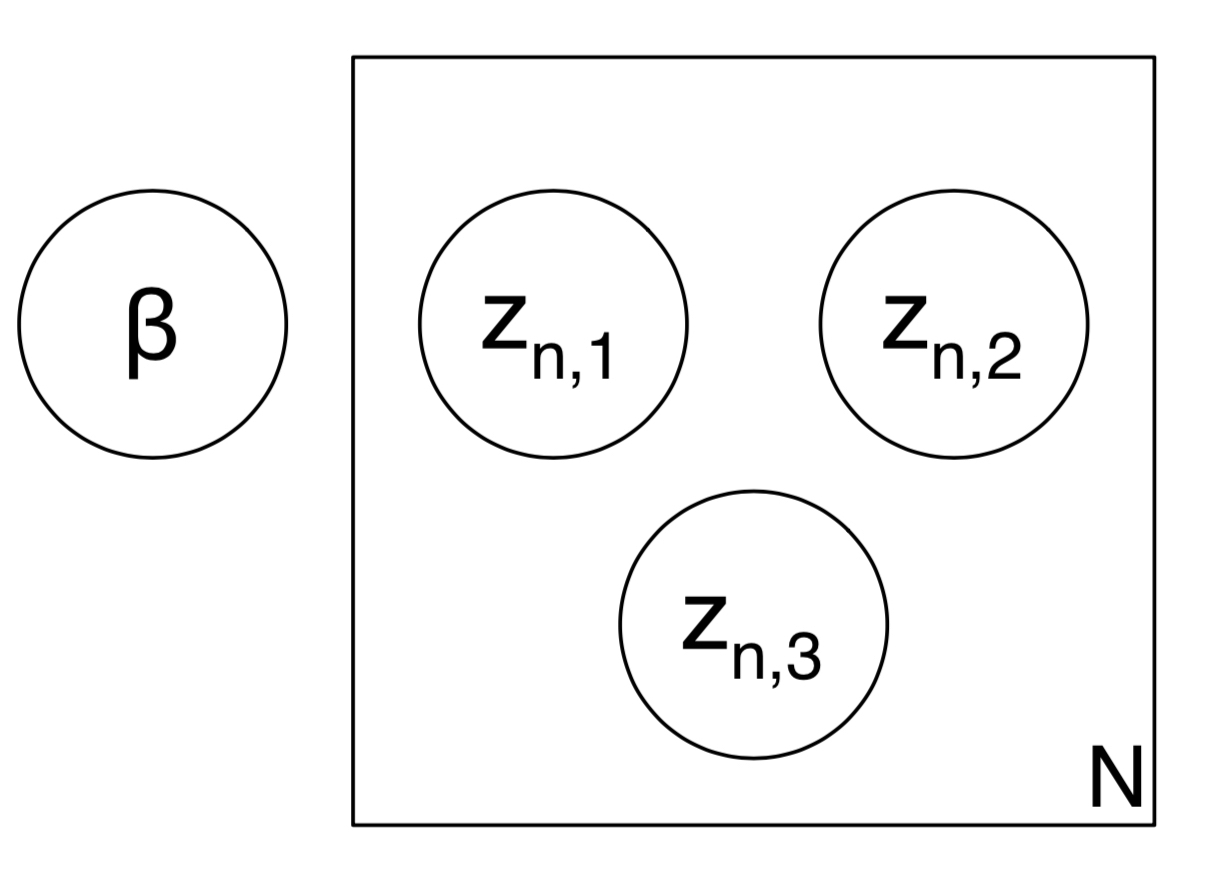
\includegraphics[width=0.8\textwidth]{mf.png}\hspace*{12cm}
        \end{figure}
    \end{column}
    \end{columns}
    \footnotetext[1]{pic from http://proceedings.mlr.press/v38/hoffman15.pdf}
\end{frame}

\begin{frame}{Variational Inference - setup}
    
    \begin{columns}
    \begin{column}{0.48\textwidth}
        \begin{figure}
        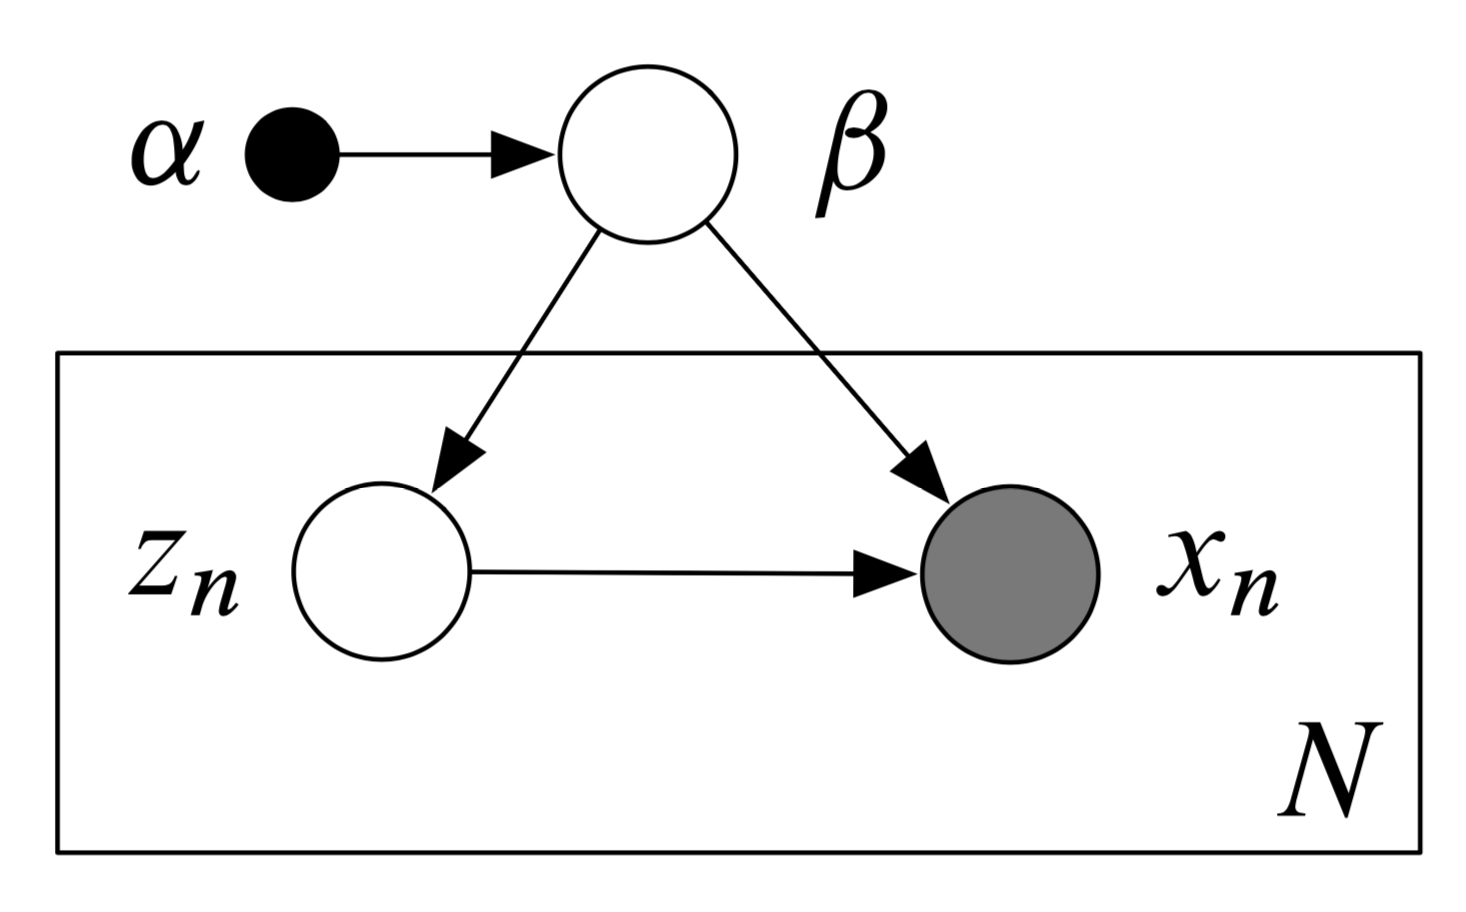
\includegraphics[width=\textwidth]{setup.png}\hspace*{12cm}
        %% add some description of this graph
        \end{figure}
    \end{column}
    \begin{column}{0.48\textwidth}
        \begin{block}{Assumptions}
        \begin{itemize}
            \item Independence of hidden variables (\textbf{Mean-Field})
            \item \textbf{Complete conditionals} are from exponential families\\
            \begin{itemize}
                \item Conditional distribution of a hidden variable given the other hidden variables and observations.
                \item $p(\beta \mid x,z)$
                \item $p(z_{nj} \mid x_n, z_{n,\backslash j},\beta)$
            \end{itemize}
        \end{itemize}
        \end{block}
    \end{column}
    \end{columns}
    \footnotetext[1]{pic from http://www.columbia.edu/~jwp2128/Papers/HoffmanBleiWangPaisley2013.pdf}
\end{frame}

\begin{frame}{Variational distribution $q$}
    \begin{itemize}
        \item Variational distribution $q$ under Mean-Field assumption
        \[q(z,\beta) = q(\beta \mid \lambda) \prod_{n=1}^N\prod_{j=1}^Jq(z_{nj} \mid \phi_{nj})\]
        \begin{itemize}
            \item $\lambda$: global variational parameters, govern global variables $\beta$
            \item $\phi_{nj}$: local variational parameters, govern $j^{th}$ local variable in the context of $n^{th}$ observation $z_{nj}$
        \end{itemize}
        \item Assumption on the form of complete conditionals \\+ conjugacy property of exponential family \\$\Rightarrow$ $q(\beta \mid \lambda)$ and $q(z_{nj} \mid \phi_{nj})$ are also from exponential families.
    \end{itemize}
\end{frame}

\begin{frame}{Evidence lower bound (ELBO)}
    \begin{itemize}
        \item Variational distributions
        \[q(\beta \mid \lambda) = \exp\{\lambda^{\top}t(\beta) - A_g(\lambda)\}\]
        \[q(z_{nj} \mid \phi_{nj}) = \exp\{\phi_{nj}^{\top}t(z_{nj}) - A_l(\phi_{nj})\}\]
        $t(\cdot)$ indicates sufficient statistics\\
        $A_{g/l}(\cdot)$ indicates global/local cumulant function
        \item \textbf{Evidence lowerbound}\\
        \[\mathcal{L}(q) = \mathbb{E}_q[\log p(x,z,\beta)] - \mathbb{E}_q[\log q(z,\beta)]\]
        \item Tradeoff between making q as spread out as possible and making q concentrate on one point that maximizes the expected log joint
    \end{itemize}
\end{frame}

\begin{frame}{Outline}

    \begin{itemize}
    \begin{greytext}
      \item A quick review of mean-field variational inference
    \end{greytext}
      \item Traditional coordinate ascent algorithm
    \begin{greytext}
      \item Stochastic variational inference(SVI)
      \item Structured SVI
      \end{greytext}
    \end{itemize}

\end{frame}

\begin{frame}{Coordinate ascent (batch)}
    \begin{itemize}
        \item Update of global variational parameters $\lambda$
         \[\nabla_{\lambda}\mathcal{L}(\lambda) = \nabla^2_{\lambda}A_g(\lambda)(\mathbb{E}_q[\eta_g(x,z)] - \lambda) = 0\]
            \[\Rightarrow \lambda = \mathbb{E}_q[\eta_g(x,z)]\]
        \item complete conditional of $\beta$
        \[p(\beta \mid x,z) = \exp\{\eta_g(x,z)^{\top}t(\beta) - A_g(\eta_g(x,z))\}\]
            \item $\eta_g(x,z)$ is the canonical parameter of $\beta$'s complete conditional distribution
        \item $\lambda$ is set to the mean parameter of $\beta$'s complete conditional distribution
         \item Similarly, for local variational parameter $\phi_{nj}$
        \[\phi_{nj} = \mathbb{E}_q[\eta_l(x_n,z_{n,\backslash j}, \beta)]\]
    \end{itemize}
\end{frame}

% \begin{frame}{Update of parameters}
%     \begin{itemize}
%         \item Similarly, for local variable $\phi_{nj}$
%         \[\phi_{nj} = \mathbb{E}_q[\eta_l(x_n,z_{n,\backslash j, \beta})]\]
%     \end{itemize}
% \end{frame}

\begin{frame}{Coordinate ascent algorithm for VI}
    \begin{block}{Coordinate ascent mean-field variational inference}
        \begin{itemize}
            \item Initialize $\lambda^{(0)}$ randomly
            \item Repeat until converges
                \begin{itemize}
                    \item for each local parameter $\phi_{nj}$
                    \begin{itemize}
                        \item set $\phi_{nj}^{(t)}$ to $\mathbb{E}_{q^{(t-1)}}[\eta_l(x_n,z_{n,\backslash j, \beta})]$     (E-step)
                    \end{itemize}
                    \item set global parameter $\lambda^{(t)}$ to $\mathbb{E}_{q^{(t)}}[\eta_g(x,z)]$     (M-step)
                \end{itemize}
        \end{itemize}
    \end{block}
    % \begin{block}{Relationship with EM}
    %     \begin{itemize}
    %         \item Update of local variational parameters corresponds to E-step
    %         \item Update of global variational parameters corresponds to M-step
    %     \end{itemize}
    % \end{block}
    \begin{block}{Problem of coordinate ascent}
        \begin{itemize}
            \item Global parameters only get updated after updating every local parameters
            % E-step takes very long time, update of each local hidden variable make use of the same global parameter we get from last iteration
            \item Wasteful if we can learn something about global parameters from a subset of data.
        \end{itemize} 
    \end{block}
\end{frame}

\begin{frame}{Outline}

    \begin{itemize}
    \begin{greytext}
      \item A quick review of mean-field variational inference
      \item Traditional coordinate ascent algorithm
    \end{greytext}
      \item Stochastic variational inference(SVI)
      \begin{itemize}
          \item Natural gradient
          \item SVI algorithm
          \item compare with coordinate ascent 
      \end{itemize}
    \begin{greytext}
      \item Structured SVI
      \end{greytext}
    \end{itemize}
\end{frame}

\begin{frame}{Natural gradient}
    %% algorithm screen shot
        \begin{itemize}
            \item Stochastic gradient ascent/descent
            \begin{itemize}
                \item Gradient computed in Euclidean space
            \end{itemize}
            \item Problem with Euclidean space when minimizing KL divergence
        \end{itemize}
    \begin{columns}
    \begin{column}{0.48\textwidth}
        \begin{figure}
        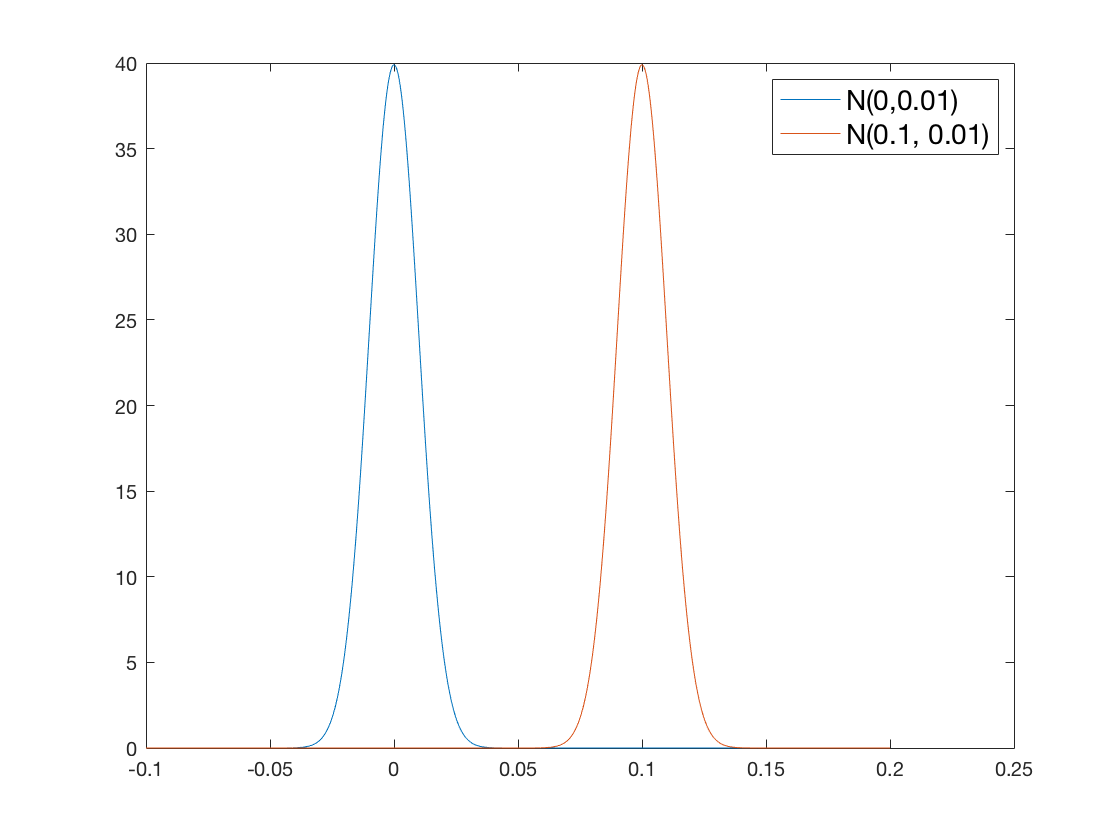
\includegraphics[width=\textwidth]{var_001.png}
        \end{figure}
    \end{column}
    \begin{column}{0.48\textwidth}
        \begin{figure}
        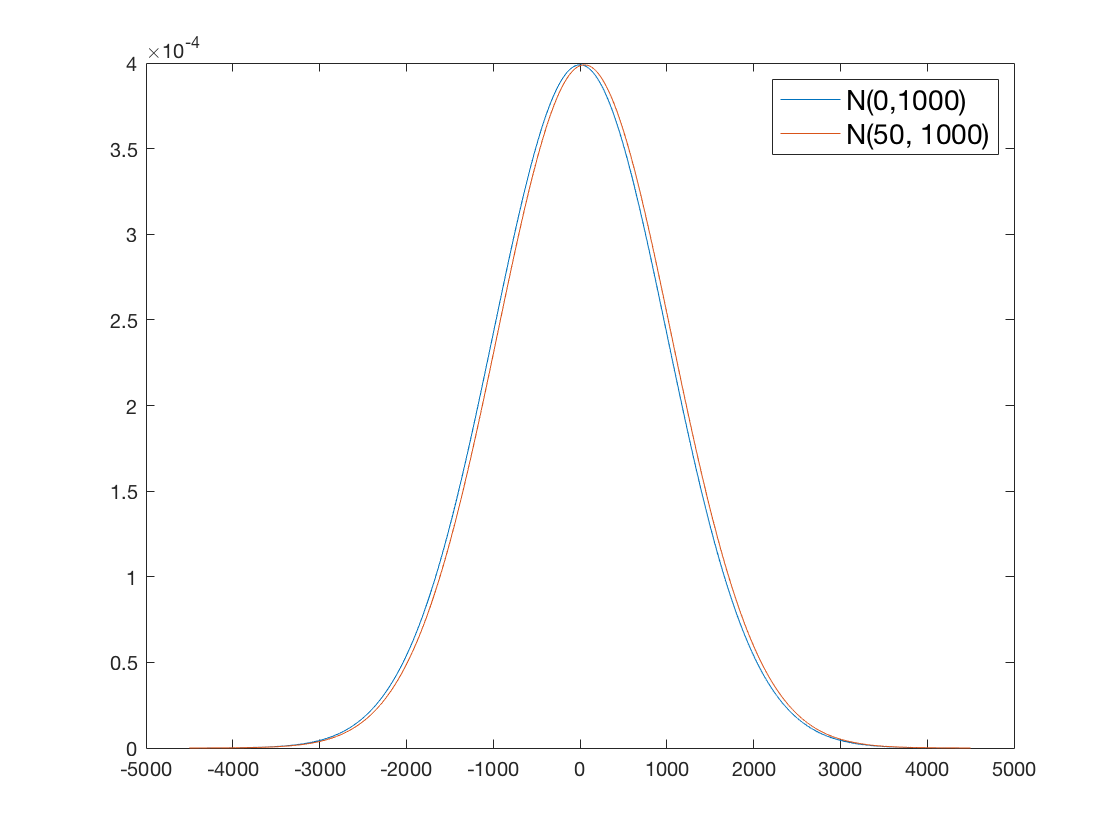
\includegraphics[width=\textwidth]{var_1000.png}
        \end{figure}
    \end{column}
    \end{columns}
\end{frame}

\begin{frame}{Natural gradient cont.}
    %% algorithm screen shot
    \begin{itemize}
        \item \textbf{Euclidean gradient}\\
        The direction of steepest ascent in \textit{Euclidean} space
        \item \textbf{Natural gradient} \\
        The direction of steepest ascent in \textit{Riemannian} space\\
        The space where distance is defined by KL divergence rather than $L2$ norm.
        \item Transform Euclidean gradient to natural gradient by left-multiplying the inverse of Riemannian metric $G(\cdot)^{-1}$
    \end{itemize}
\end{frame}



\begin{frame}{Natural gradient cont.}
    %% algorithm screen shot
    \begin{itemize}
        \item Natural gradient of global variational parameters (similarly for local variational parameters)
        \[\hat{\nabla}_{\lambda}\mathcal{L}(\lambda) = G(\lambda)^{-1}\nabla_{\lambda}\mathcal{L}(\lambda)\]
         $G(\lambda)$ is the second derivative of the log partition of $q(\beta \mid \lambda)$
         \[G(\lambda) = \nabla^2_{\lambda}A_g(\lambda)\]
        \item In the coordinate ascent section, we have derived the gradient of ELBO w.r.t. $\lambda$
        \[\nabla_{\lambda}\mathcal{L}(\lambda) = \nabla^2_{\lambda}A_g(\lambda)(\mathbb{E}_q[\eta_g(x,z)] - \lambda)\]
        \item The natural gradient of $\lambda$ is thus
        \[\hat{\nabla}_{\lambda}\mathcal{L}(\lambda) = \mathbb{E}_q[\eta_g(x,z)] - \lambda \]
    \end{itemize}
\end{frame}

\begin{frame}{Stochastic variational inference}
    \begin{itemize}
        \item Rewrite ELBO to global term and sum of local terms
        \begin{align*}
            \mathcal{L}(q) &= \mathbb{E}_q[\log p(x,z,\beta)] - \mathbb{E}_q[\log q(z,\beta)]\\
            &= \mathbb{E}_q[\log \frac{p(\beta)}{q(\beta)}] + \sum\limits_{n=1}^N \mathbb{E}_q[\log \frac{p(z_n, x_n \mid \beta)}{q(z_n)}]
        \end{align*}
        \item Sample one $x_i$ uniformly from the data set and duplicate N times as the sum of local terms
        \[\mathcal{L}_I(q) = \mathbb{E}_q[\log \frac{p(\beta)}{q(\beta)}] + N \mathbb{E}_q[\log \frac{p(z_i, x_i \mid \beta)}{q(z_i)}]\]
        \item Natural gradient of $\mathcal{L}_I$ w.r.t $\lambda$ is noisy but unbiased, because %(view ELBO as a function of global variational parameter $\lambda$)
        \[\mathbb{E}[\mathcal{L}_I(\lambda)] = \mathcal{L}(\lambda)\]
    \end{itemize}
\end{frame}

\begin{frame}{Stochastic variational inference}
    \begin{itemize}
        \item Let $\{x_i^{(N)}, z_i^{(N)}\}$ be a set of $N$ replicates of $x_i$ and $z_i$
        \item Noisy natural gradient of ELBO
        \[\hat{\nabla}_{\lambda}\mathcal{L}_I(\lambda) = \mathbb{E}_q[\eta_g(x_i^{(N)}, z_i^{(N)})] - \lambda\]
        \item Define intermediate global parameter $\hat{\lambda_i}$
        \[\hat{\nabla}_{\lambda}\mathcal{L}_I(\lambda) = 0\]
        \[\hat{\lambda_i} = \mathbb{E}_q[\eta_g(x_i^{(N)}, z_i^{(N)})] = N\mathbb{E}_q[\eta_g(x_i, z_i)]\]
        A noisy estimate of $\lambda$ using only one point, easy to compute
        
    \end{itemize}
\end{frame}

\begin{frame}{Stochastic variational inference}
    \begin{itemize}
        \item $\lambda^{(t-1)}$: estimate of global parameters in previous step\\ $\hat{\lambda}_t$: intermediate global estimate of current step
        \item Let $\rho_t$ be the step size at time $t$
        \begin{align*}
            \lambda^{(t)} &=
            \lambda^{(t-1)} + \rho_t(\hat{\lambda}_t - \lambda^{(t-1)})\\
            &= (1-\rho_t)\lambda^{(t-1)} + \rho_t\hat{\lambda}_t
        \end{align*}
        \begin{itemize}
            \item since \[\mathbb{E}[\hat{\lambda}_t - \lambda^{(t-1)}] = \mathbb{E}[\hat{\nabla}_{\lambda}\mathcal{L}_{I}(\lambda)] =  \nabla_{\lambda}\mathcal{L}(\lambda)\]
        \end{itemize}
        \item Global parameter $\lambda^{(t)}$ is the weighted average between previous $\lambda^{(t-1)}$ and estimate of $\lambda$ if the sampled data point was replicated N times.
        
    \end{itemize}
\end{frame}


\begin{frame}{Stochastic variational Inference}
    \begin{block}{Steps:}
        \textbf{Repeat} until converges
        \begin{enumerate}
            \item Sample data point $x_i$ uniformly from the data set
            \item Update local variational parameters $\phi_{ij}$ to $\mathbb{E}_{q^{(t-1)}}[\eta_l(x_i, \beta, z_{i,\backslash j})]$
            \item Compute intermediate estimate of global variational parameter by duplicating N times of a point $\hat{\lambda}_t = \mathbb{E}_q[\eta_g(x_i^{(N)}, z_i^{(N)})]$
            \item Update global parameter using weighted average $\lambda^{(t)} = (1-\rho_t)\lambda^{(t-1)} + \rho_t\hat{\lambda}_t$
    \end{enumerate}
    \end{block}
\end{frame}

\begin{frame}{Stochastic variational Inference - LDA experiment}
    \begin{figure}
        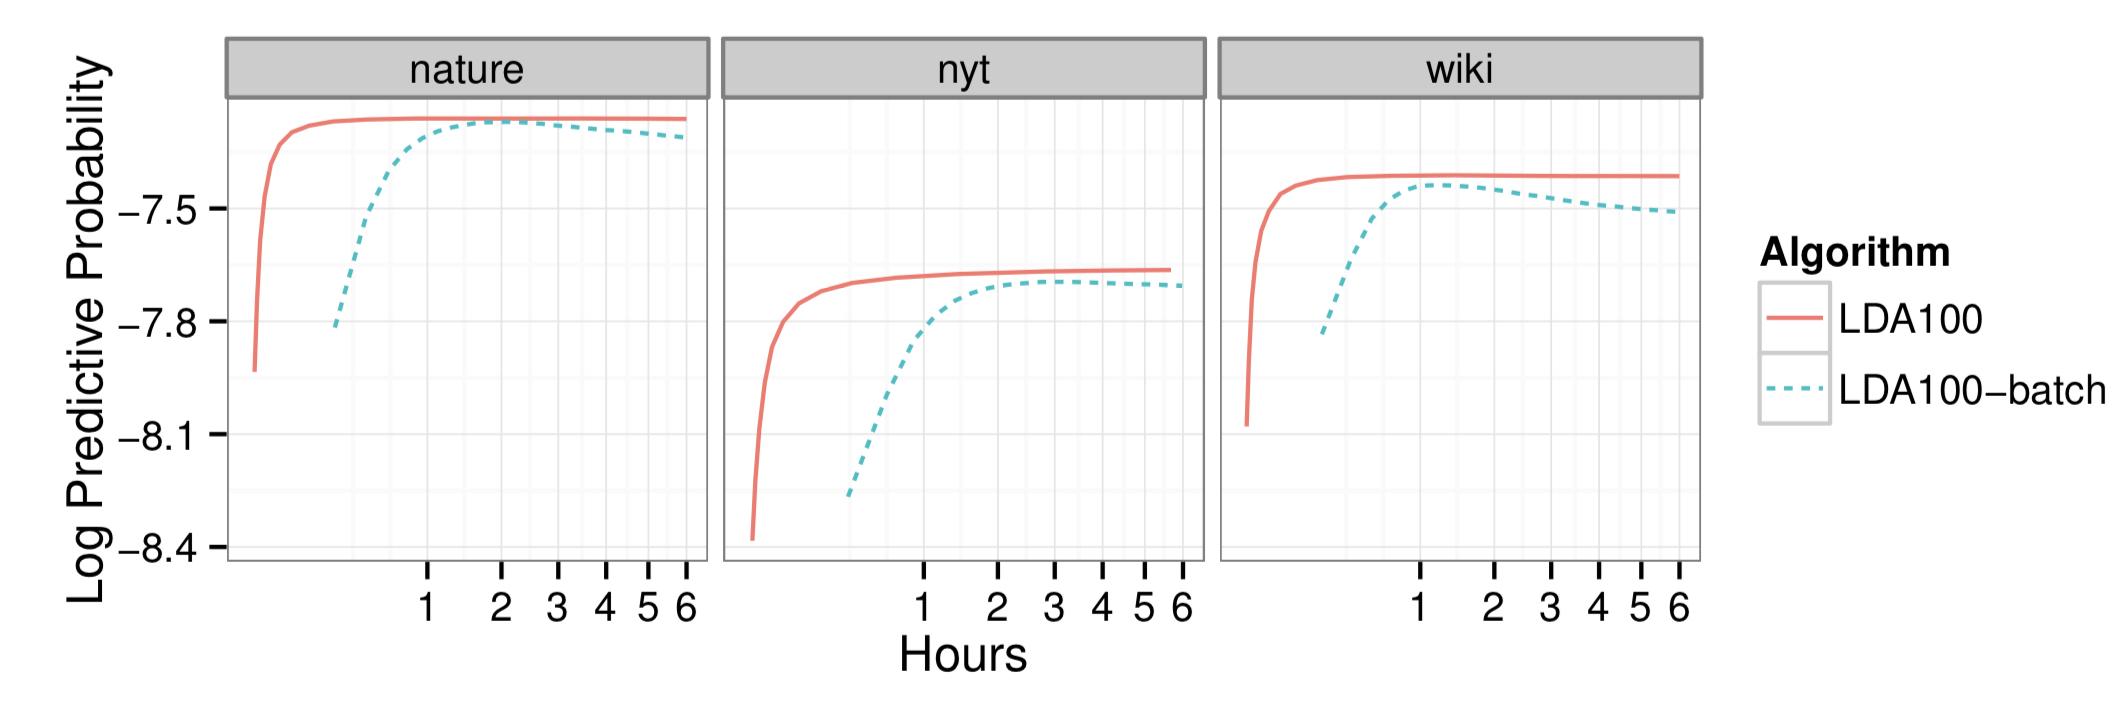
\includegraphics[width=\textwidth]{LDA_SVI.png}
    \end{figure}
    \begin{itemize}
        \item Per-word predictive log likelihood for 100-topic LDA model on 3 large corpora.
        \item Split each document to observed words (obs) and held out words (new); compute $p(w_{new} \mid w_{obs}, \mathcal{D})$
        \item SVI converges faster and to a better place
    \end{itemize}
\end{frame}

\begin{frame}{Outline}

    \begin{itemize}
    \begin{greytext}
      \item A quick review of mean-field variational inference
      \item Traditional coordinate ascent algorithm
      \item Stochastic variational inference(SVI)
    \end{greytext}
      \item Structured SVI
    \end{itemize}
\end{frame}


\begin{frame}{Structured SVI}
    \begin{itemize}
        \item Mean-Field assumption of SVI\\
        Hidden variables are all independent of each other\\
        Although easier to compute, it becomes less likely to approximate the correct $p(z, \beta \mid x)$
        \item\textbf{ Structured stochastic variational inference}\\
        Allow arbitrary dependencies between global and local variables
    \end{itemize}
\end{frame}

\begin{frame}{Structured SVI}
    %% algorithm screen shot
    \begin{columns}
    \begin{column}{0.48\textwidth}
        \begin{figure}
        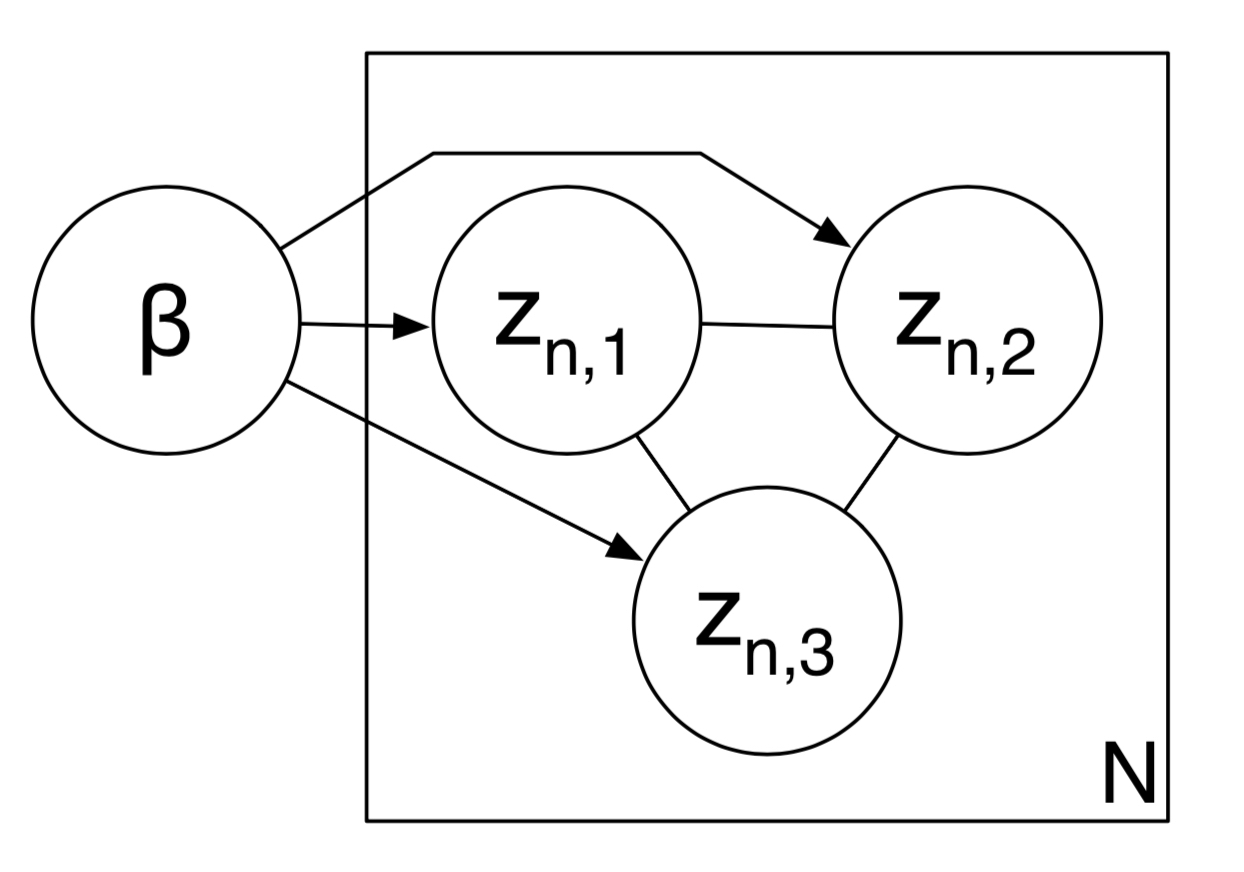
\includegraphics[width=\textwidth]{structured_mf.png}\hspace*{12cm}
        %% add some description of this graph
        \end{figure}
    \end{column}
    \begin{column}{0.48\textwidth}
        \begin{block}{Hidden structure}
        \[q(z, \beta) = q(\beta \mid \lambda) \prod\limits_{n=1}^N q(z_n \mid \gamma_n(\beta))\]
        $\gamma_n(\beta)$ is a vector-valued function, represents any possible dependencies between $z_n$ and $\beta$
        \end{block}
    \end{column}
    \end{columns}
\end{frame}

\begin{frame}{Structured SVI}
    \begin{itemize}
        \item Require $p(\beta)$ and $p(x_n, z_n \mid \beta)$ are from exponential families and having the form
        \[p(\beta) = \exp\{\eta^{\top} t(\beta) - A_g(\eta)\}\]
        \[p(x_n, z_n \mid \beta) = \exp\{\eta_n(x_n, z_n)^{\top}t(\beta) + g_n(x_n, z_n)\}\]
        $\eta_n(x_n, z_n)$ is a vector-valued function%, $g_n$ is a scalar-valued function
        \item Weakened assumption: do not require exponential form or tractability of the complete conditionals of local hidden variables
        % \item The most general distribution 
        % \[p(\beta \mid x,z) = \exp\{(\eta + \sum_n\eta_n(x_n,z_n))^{\top}t(\beta) - A_g(\eta + \sum_n\eta_n(x_n,z_n))\}\]
    \end{itemize}
\end{frame}

\begin{frame}{Structured SVI}
    \begin{block}{SSVI steps:}
        \textbf{Repeat} until converges
        \begin{enumerate}
            \item Sample global variable $\beta^{(t)}$ from $q(\beta \mid \lambda^{(t-1)})$
            \item Compute local variational parameters $\gamma_n(\beta^{(t)})$ which maximizes local ELBO
            $\mathbb{E}_q[\log p(x_n, z_n \mid \beta) - \log q(z_n \mid \beta)]$
            
            \begin{itemize}
                \begin{greytext}
                \item \textit{analogous to updating local variational parameter $\phi_{nj}$ in SVI}
                \end{greytext}
            \end{itemize}
            
            \item Update $\hat{\eta}_n$ to be $\mathbb{E}[\eta_n(x_n, z)] = \sum_{z_n}q(z_n \mid \gamma_n(\beta^{(t)}))\eta_n(x_n,z_n)$%, weighted average of the vector-valued function of the local joint distribution given global parameters.
            
            \begin{itemize}
            \begin{greytext}
                \item contribution of $n^{th}$ local context to the update of global parameters
                \item \textit{analogous to computing noisy estimate of global parameter in SVI}
                \end{greytext}
            \end{itemize}
            
            
            \item Update $\lambda^{(t)}$ to be the weighted average of previous $\lambda^{(t-1)}$ and noisy estimate
            
            \begin{itemize}
                \begin{greytext}
                \item \textit{Standard Robbins-Monro algorithm}
                \end{greytext}
            \end{itemize}
            
            
        \end{enumerate}
    \end{block}
\end{frame}

\begin{frame}{Structured SVI}
    \begin{figure}
        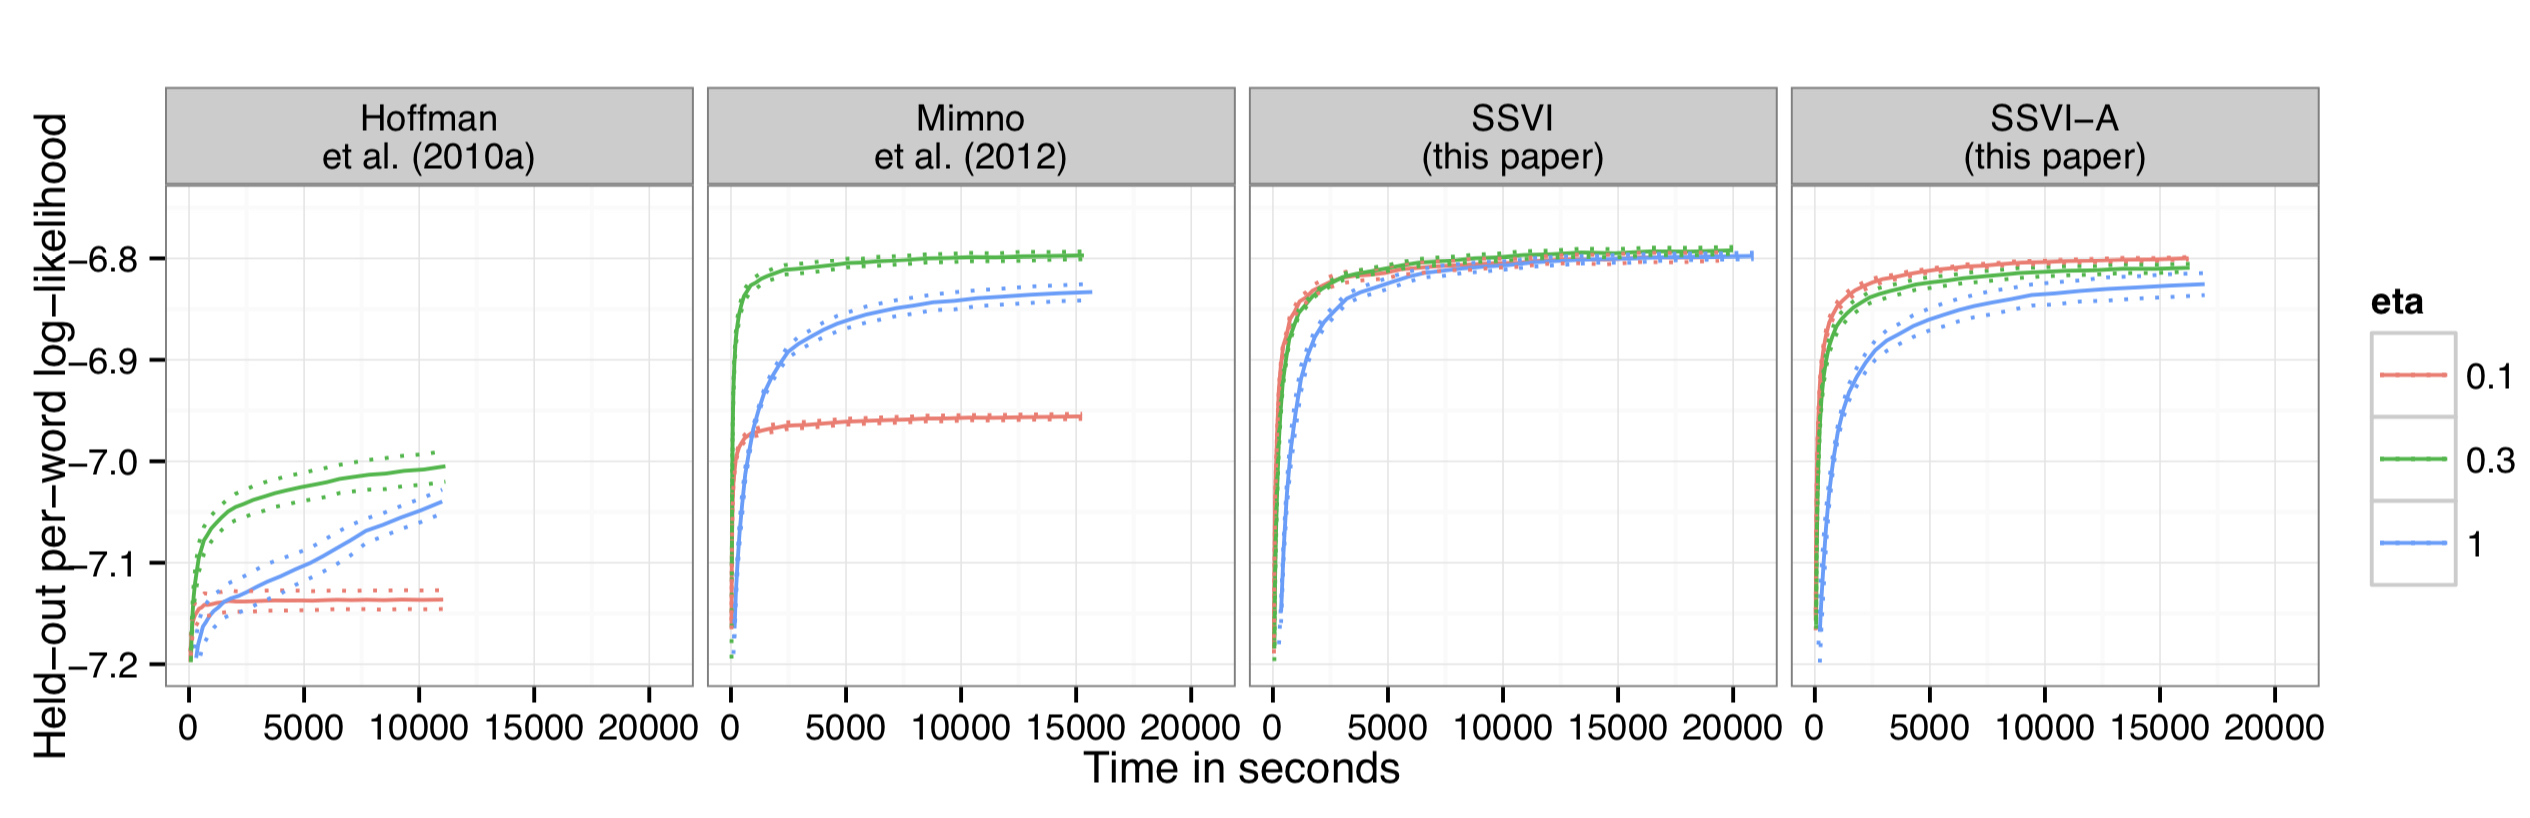
\includegraphics[width=\textwidth]{SSVI.png}
    \end{figure}
    \begin{itemize}
        \item Wiki copora, per-word log likelihood
        \item SSVI-A: same procedure, simplfied version of noisy estimate
        \item SSVI converge to better place than SVI with mean field assumption
        \item SSVI is less sensitive to the chosen hyper-parameters
    \end{itemize}
\end{frame}

\begin{frame}{QA}
    Questions?
\end{frame}



\end{document}
